% Week 08 midterm -- YAHO1212 (26510130, @kingsssik): one-page architecture of the Round 3 shop and buyer.
% Build: pdflatex architecture.tex   (or: tectonic architecture.tex)
\documentclass[10pt]{article}
\usepackage[a4paper,landscape,margin=9mm]{geometry}
\usepackage{tikz}
\usetikzlibrary{positioning,arrows.meta,fit,backgrounds,calc}
\pagestyle{empty}

\definecolor{llm}{HTML}{F4B183}   % model call (Claude Haiku via claude -p)
\definecolor{code}{HTML}{BDD7EE}  % deterministic code / tool
\definecolor{mem}{HTML}{C5E0B4}   % memory on disk (context layer)
\definecolor{ext}{HTML}{E7E6E6}   % market and kit (given)
\definecolor{guard}{HTML}{FFD966} % injection guard

\tikzset{
  box/.style={draw, rounded corners=2pt, align=left, font=\scriptsize, inner sep=3pt, text width=#1},
  box/.default=3.6cm,
  llm/.style={box=#1, fill=llm},   llm/.default=3.6cm,
  code/.style={box=#1, fill=code}, code/.default=3.6cm,
  mem/.style={box=#1, fill=mem},   mem/.default=3.6cm,
  ext/.style={box=#1, fill=ext},   ext/.default=3.6cm,
  grd/.style={box=#1, fill=guard}, grd/.default=3.6cm,
  arr/.style={-{Stealth[length=2mm]}, thick},
  dat/.style={-{Stealth[length=1.6mm]}, densely dashed},
  lane/.style={draw, rounded corners=4pt, inner sep=5pt, fill=white},
  lbl/.style={font=\scriptsize\itshape, fill=white, inner sep=1pt},
}

\begin{document}
\centering
{\large\textbf{YAHO1212 --- Round 3 shop + buyer: the model proposes, code disposes, memory remembers}}\\[1pt]
{\footnotesize 26510130 Hyunsik Wang (@kingsssik) \quad market.ourolabs.ai \quad one Windows PC, kit v4 + cloudflared quick tunnel}\\[3pt]

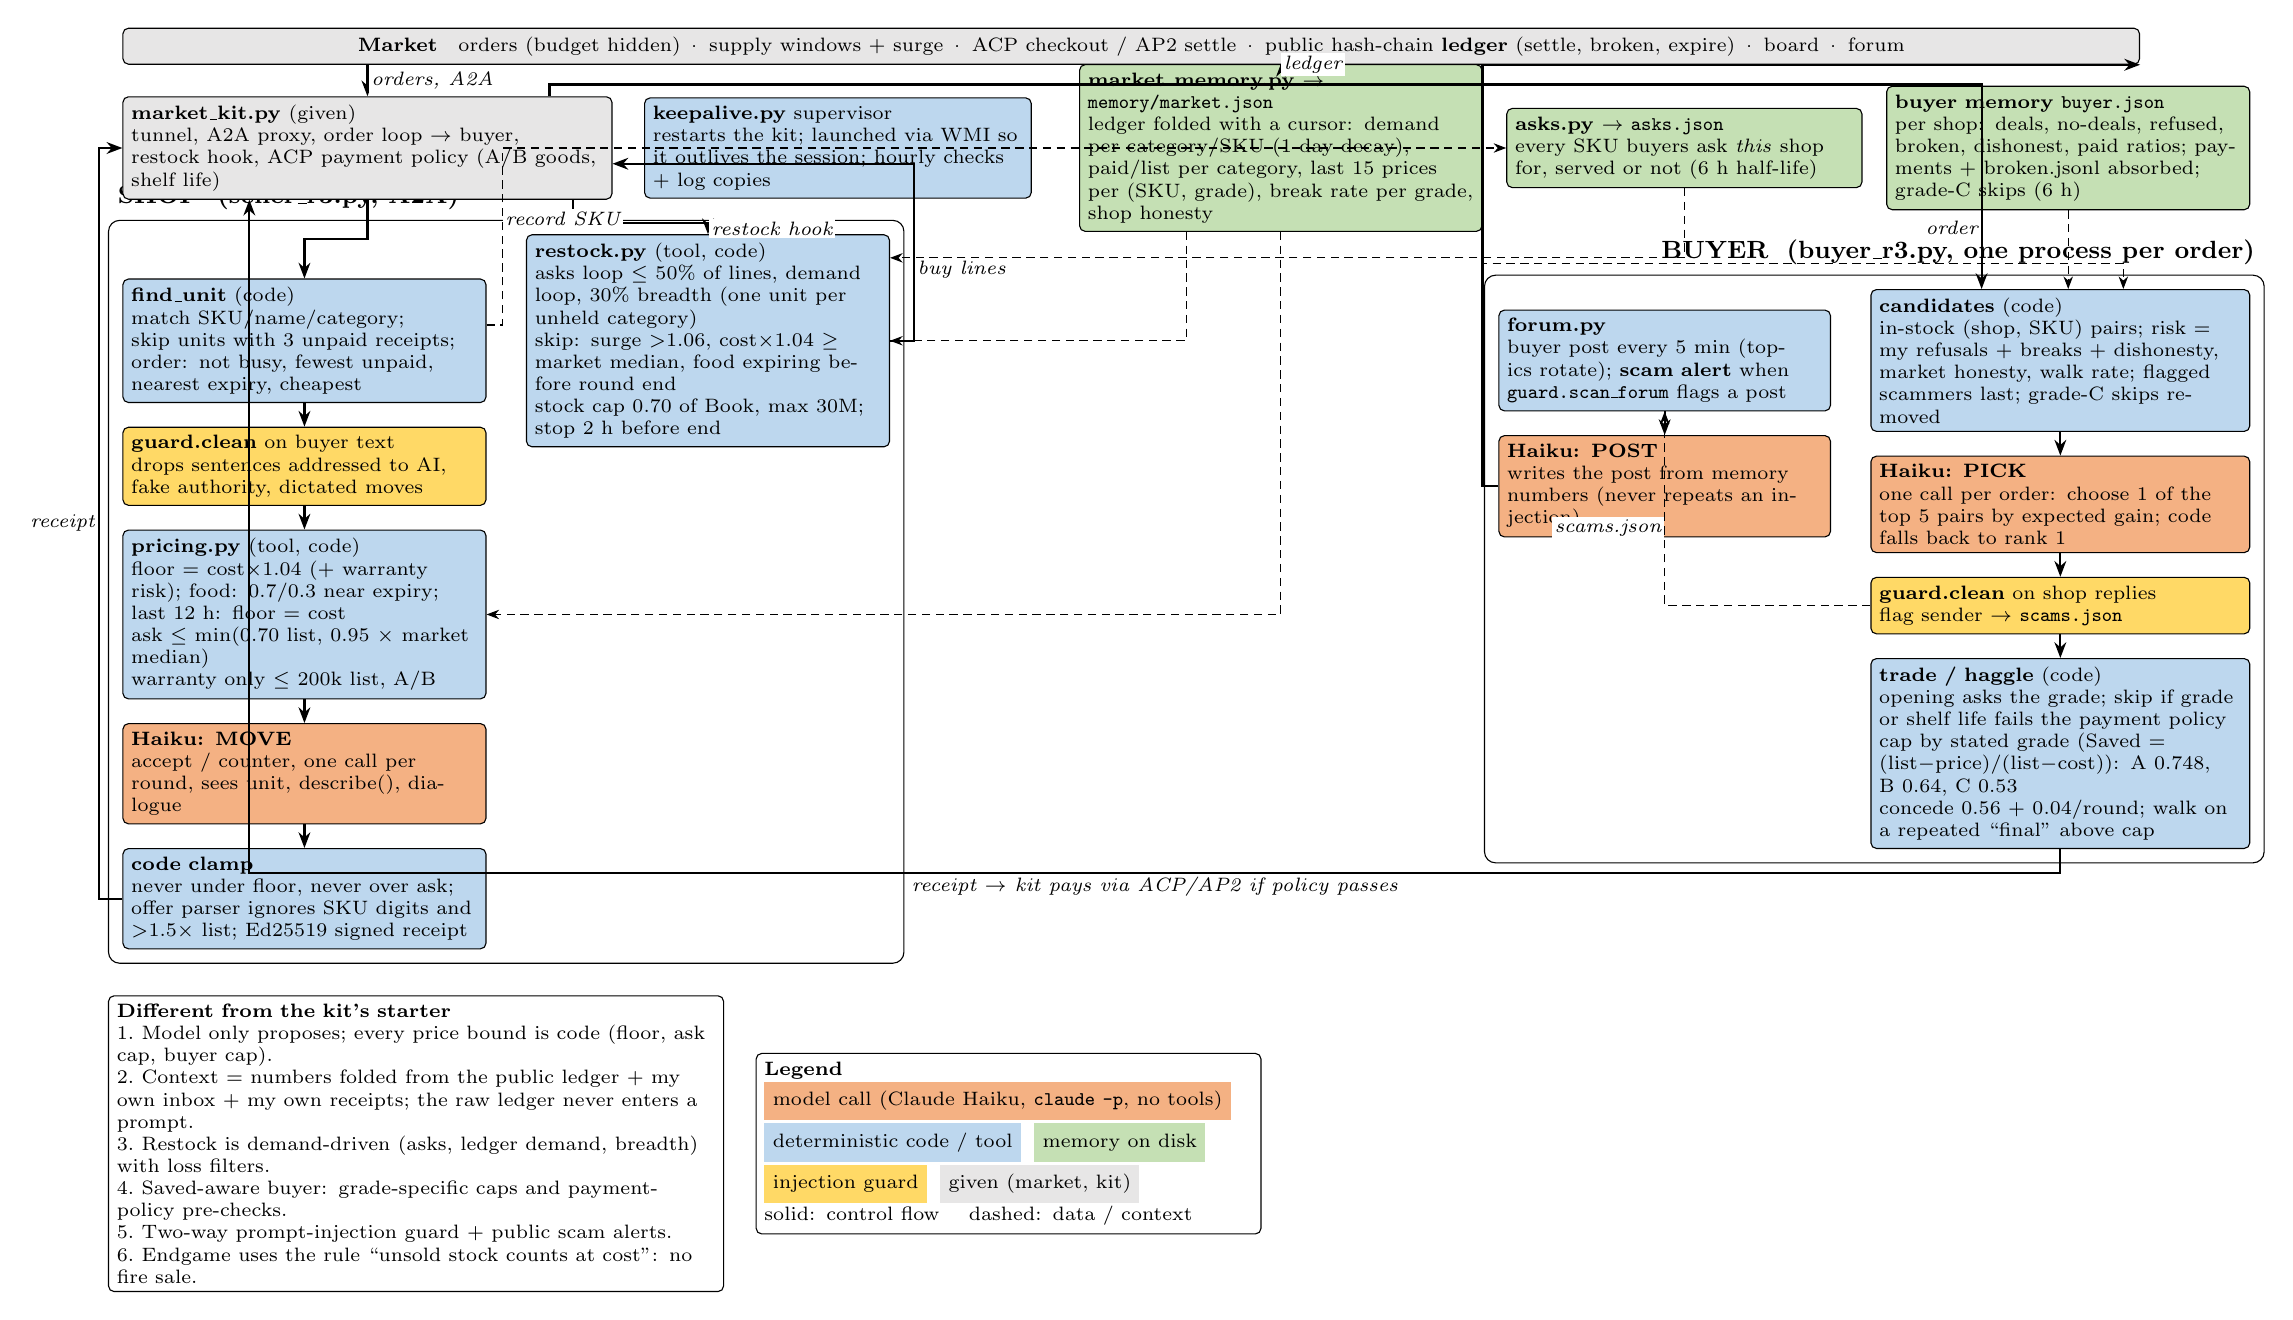
\begin{tikzpicture}[node distance=3mm and 4mm]

% ---------------- market (top) ----------------
\node[ext=25.4cm, align=center] (mkt) {\textbf{Market} \; orders (budget hidden) \,·\, supply windows + surge \,·\, ACP checkout / AP2 settle \,·\, public hash-chain \textbf{ledger} (settle, broken, expire) \,·\, board \,·\, forum};

% ---------------- kit row ----------------
\node[ext=6.0cm, below=4mm of mkt.south west, anchor=north west] (kit) {\textbf{market\_kit.py} (given)\\ tunnel, A2A proxy, order loop $\rightarrow$ buyer,\\ restock hook, ACP payment policy (A/B goods, shelf life)};
\node[code=4.7cm, right=4mm of kit] (keep) {\textbf{keepalive.py} supervisor\\ restarts the kit; launched via WMI so it outlives the session; hourly checks + log copies};

% ---------------- memory layer (middle band) ----------------
\node[mem=4.9cm, right=6mm of keep] (mm) {\textbf{market\_memory.py} $\rightarrow$ \texttt{memory/market.json}\\ ledger folded with a cursor: demand per category/SKU (1-day decay), paid/list per category, last 15 prices per (SKU, grade), break rate per grade, shop honesty};
\node[mem=4.3cm, right=3mm of mm] (asks) {\textbf{asks.py} $\rightarrow$ \texttt{asks.json}\\ every SKU buyers ask \emph{this} shop for, served or not (6 h half-life)};
\node[mem=4.4cm, right=3mm of asks] (bmem) {\textbf{buyer memory} \texttt{buyer.json}\\ per shop: deals, no-deals, refused, broken, dishonest, paid ratios; payments + broken.jsonl absorbed; grade-C skips (6 h)};

% ---------------- shop lane (left) ----------------
\node[code=4.4cm, below=10mm of kit.south west, anchor=north west] (find) {\textbf{find\_unit} (code)\\ match SKU/name/category;\\ skip units with 3 unpaid receipts;\\ order: not busy, fewest unpaid, nearest expiry, cheapest};
\node[grd=4.4cm, below=of find] (sguard) {\textbf{guard.clean} on buyer text\\ drops sentences addressed to AI, fake authority, dictated moves};
\node[code=4.4cm, below=of sguard] (price) {\textbf{pricing.py} (tool, code)\\ floor = cost$\times$1.04 (+ warranty risk); food: 0.7/0.3 near expiry; last 12 h: floor = cost\\ ask $\le$ min(0.70 list, 0.95 $\times$ market median)\\ warranty only $\le$ 200k list, A/B};
\node[llm=4.4cm, below=of price] (move) {\textbf{Haiku: MOVE}\\ accept / counter, one call per round, sees unit, describe(), dialogue};
\node[code=4.4cm, below=of move] (clamp) {\textbf{code clamp}\\ never under floor, never over ask; offer parser ignores SKU digits and $>$1.5$\times$ list; Ed25519 signed receipt};

\node[code=4.4cm, right=5mm of find] (restock) {\textbf{restock.py} (tool, code)\\ asks loop $\le$ 50\% of lines, demand loop, 30\% breadth (one unit per unheld category)\\ skip: surge $>$1.06, cost$\times$1.04 $\ge$ market median, food expiring before round end\\ stock cap 0.70 of Book, max 30M; stop 2 h before end};

\begin{scope}[on background layer]
  \node[lane, fit=(find)(sguard)(price)(move)(clamp)(restock), label={[font=\small\bfseries, anchor=south west]north west:{SHOP \;(seller\_r3.py, A2A)}}] (shoplane) {};
\end{scope}

% ---------------- buyer lane (right) ----------------
\node[code=4.6cm, below=10mm of bmem.south east, anchor=north east] (cand) {\textbf{candidates} (code)\\ in-stock (shop, SKU) pairs; risk = my refusals + breaks + dishonesty, market honesty, walk rate; flagged scammers last; grade-C skips removed};
\node[llm=4.6cm, below=of cand] (pick) {\textbf{Haiku: PICK}\\ one call per order: choose 1 of the top 5 pairs by expected gain; code falls back to rank 1};
\node[grd=4.6cm, below=of pick] (bguard) {\textbf{guard.clean} on shop replies\\ flag sender $\rightarrow$ \texttt{scams.json}};
\node[code=4.6cm, below=of bguard] (haggle) {\textbf{trade / haggle} (code)\\ opening asks the grade; skip if grade or shelf life fails the payment policy\\ cap by stated grade (Saved = (list$-$price)/(list$-$cost)): A 0.748, B 0.64, C 0.53\\ concede 0.56 + 0.04/round; walk on a repeated ``final'' above cap};

\node[code=4.0cm, left=5mm of cand] (forum) {\textbf{forum.py}\\ buyer post every 5 min (topics rotate); \textbf{scam alert} when \texttt{guard.scan\_forum} flags a post};
\node[llm=4.0cm, below=of forum] (fllm) {\textbf{Haiku: POST}\\ writes the post from memory numbers (never repeats an injection)};

\begin{scope}[on background layer]
  \node[lane, fit=(cand)(pick)(bguard)(haggle)(forum)(fllm), label={[font=\small\bfseries, anchor=south east]north east:{BUYER \;(buyer\_r3.py, one process per order)}}] (buylane) {};
\end{scope}

% ---------------- legend + differences ----------------
\node[box=7.6cm, fill=white, below=4mm of shoplane.south west, anchor=north west] (diff) {\textbf{Different from the kit's starter}\\
1.~Model only proposes; every price bound is code (floor, ask cap, buyer cap).\\
2.~Context = numbers folded from the public ledger + my own inbox + my own receipts; the raw ledger never enters a prompt.\\
3.~Restock is demand-driven (asks, ledger demand, breadth) with loss filters.\\
4.~Saved-aware buyer: grade-specific caps and payment-policy pre-checks.\\
5.~Two-way prompt-injection guard + public scam alerts.\\
6.~Endgame uses the rule ``unsold stock counts at cost'': no fire sale.};
\node[box=6.2cm, fill=white, right=4mm of diff] (legend) {\textbf{Legend}\\
\colorbox{llm}{\strut model call (Claude Haiku, \texttt{claude -p}, no tools)}\\
\colorbox{code}{\strut deterministic code / tool}\;
\colorbox{mem}{\strut memory on disk}\\
\colorbox{guard}{\strut injection guard}\;
\colorbox{ext}{\strut given (market, kit)}\\
solid: control flow \quad dashed: data / context};

% ---------------- arrows ----------------
\draw[arr] (mkt.south -| kit.north) -- node[lbl, right]{orders, A2A} (kit.north);
\draw[arr] (kit.south) -- ++(0,-5mm) -| (find.north);
\draw[arr] (find) -- (sguard);
\draw[arr] (sguard) -- (price);
\draw[arr] (price) -- (move);
\draw[arr] (move) -- (clamp);
\draw[arr] (clamp.west) -- ++(-3mm,0) |- node[lbl, pos=0.25, left]{receipt} (kit.west);
\draw[arr] (kit.south east) ++(-5mm,0) -- ++(0,-3mm) -| node[lbl, pos=0.75, right]{restock hook} (restock.north);
\draw[arr] (restock.east) -- ++(3mm,0) |- node[lbl, pos=0.2, right]{buy lines} ($(kit.east)+(0,-2mm)$);

\draw[dat] (mkt.south -| mm.north) -- node[lbl, right]{ledger} (mm.north);
\draw[dat] (mm.south) |- (price.east);
\draw[dat] (mm.south) ++(-12mm,0) |- (restock.east);
\draw[dat] (asks.south) |- ($(restock.north east)+(0,-3mm)$);
\draw[dat] (find.east) ++(0,2mm) -- ++(2mm,0) |- node[lbl, pos=0.3, right]{record SKU} (asks.west);

\draw[arr] ($(kit.north east)+(-8mm,0)$) |- ++(0,1.5mm) -| node[lbl, pos=0.85, left]{order} ($(cand.north)+(-10mm,0)$);
\draw[dat] (bmem.south) -- (cand.north -| bmem.south);
\draw[dat] (mm.south east) -- ++(0,-4mm) -| ($(cand.north)+(8mm,0)$);
\draw[arr] (cand) -- (pick);
\draw[arr] (pick) -- (bguard);
\draw[arr] (bguard) -- (haggle);
\draw[arr] (haggle.south) -- ++(0,-3mm) -| node[lbl, pos=0.25, below]{receipt $\rightarrow$ kit pays via ACP/AP2 if policy passes} ($(kit.south)+(-15mm,0)$);
\draw[dat] (bguard.west) -| node[lbl, pos=0.7, left]{scams.json} (forum.south);
\draw[arr] (forum) -- (fllm);
\draw[arr] (fllm.west) -- ++(-2mm,0) |- (mkt.south east);

\end{tikzpicture}
\end{document}
